%%%%%%%%%%%%%%%%%%%%%%%%%%%%%%%%%%%%%%%%%%%%%%%%%%%%%%%%
%%%%%%%%%%%%%%%%%%%%%%%%%%%%%%%%%%%%%%%%%%%%%%%%%%%%%%%%
\chapter{Regression}
\label{chap:regression}

%%%%%%%%%%%%%%%%%%%%%%%%%%%%%%%%%%%%%%%%%%%%%%%%%%%%%%%%
%%%%%%%%%%%%%%%%%%%%%%%%%%%%%%%%%%%%%%%%%%%%%%%%%%%%%%%%
\section{Linear Regression}
\label{regression:linear}

Linear regression fits the best hyperplane, or line in 1D,
to a collection of $m$ points $\mathbf{x}_{i}, y_{i}$,
typically via the method of least squares.
If $\mathbf{x}$ has $n$ features we can represent the
linear relationship between $\mathbf{x}$ and $y$ as:

\begin{equation}\label{eq:linear:onepoint}
y_{i} = \beta_{0} + \sum_{j=1}^{n}\, \beta_{j} x_{ij} + \epsilon_{i}\,,
\end{equation}

\noindent where $\beta_{j}$ are the parameters of the regression
and $\epsilon$ represent random errors.
Transitioning to matrix notation\footnote{Note
that \textit{linear} regression refers to the linearity in the model parameters
$\bm{\beta}$, not $\mathbf{X}$.
The components of $\mathbf{X}_{i}$ can be, and often are,
non-linear functions of other input features.}, this is simply:

\begin{equation}\label{eq:linear:matrix}
\mathbf{y} = \mathbf{X} \bm{\beta} + \bm{\epsilon}\,,
\end{equation}

\noindent where we have set $X_{i0} =1$.

The ordinary least squares (OLS) estimate of the parameters $\hat{\bm{\beta}}$
can be found by minimizing the squares of the residuals,
\ie the objective function $S\left(\bm{\beta}\right)$:

\begin{subequations} \label{eq:linear:ols}
\begin{align}
\hat{\bm{\beta}} &= \argmin_{\bm{\beta}} S\left(\bm{\beta}\right)\,, \label{eq:linear:argmin} \\
S\left(\bm{\beta}\right) &= \sum_{i=1}^{m} \, \abs{y_{i} - \sum_{j=0}^{n} \, \beta_{j} x_{ij}}^{2} = \norm{\mathbf{y} - \mathbf{X} \bm{\beta}}^{2}\,. \label{eq:linear:S}
\end{align}
\end{subequations}

\noindent The optimal $\hat{\bm{\beta}}$ of \cref{eq:linear:ols} has a closed form solution:

\begin{equation}\label{eq:linear:betahat}
\hat{\bm{\beta}} = \left(\mathbf{X}\transpose\mathbf{X}\right)^{-1}\mathbf{X}\transpose \mathbf{y}\,,
\end{equation}

\noindent provided the following assumptions hold:

%%%%%%%%%%%%%%%%%%%%%%%%%%%%%%%%%%%%%%%%%%%%%%%%%%%%%%%%
\subsection{Assumptions}
\label{regression:linear:assumptions}

\begin{enumerate}[noitemsep]
\item The underlying relationship between $\mathbf{x}$ and $y$ is linear, and there are no major outliers.\label{item:regression:linear:linear}
\item The columns of $\mathbf{X}$, \ie features, are linearly independent, \ie $\mathrm{rank}\left(\mathbf{X}\right) = n$ (no multicollinearity).\label{item:regression:linear:multicollinearity}
\item The errors $\epsilon$ have conditional mean 0, $E\left(\epsilon \mid \mathbf{X}\right) = 0$ (exogeneity). The errors thus:\label{item:regression:linear:exogeneity}
\begin{enumerate}[noitemsep]
\item Have a mean of zero, $E\left(\epsilon\right) = 0$.
\item Are not correlated with the input features, $E\left(\mathbf{X}\transpose\epsilon\right) = 0$.
\end{enumerate}
\item The errors are spherical, $\mathrm{var}\left(\epsilon \mid \mathbf{X}\right) = \sigma^{2} \identity$. Thus:\label{item:regression:linear:spherical}
\begin{enumerate}[noitemsep]
\item Each observation $\mathbf{x}_{i}$ has the same constant variance $\sigma^{2}$ (homoscedasticity).
\item The errors are uncorrelated between observations, $E\left(\epsilon_{i}\epsilon_{j \neq i} \mid \mathbf{X}\right) = 0$ (no autocorrelation).
\end{enumerate}
\item The errors are normally distributed (multivariate normality)\footnote{This is not strictly required, but if true the OLS is the MLE and hypothesis testing works.}.\label{item:regression:linear:normality}
\end{enumerate}

If these assumptions are violated the following issues arise,
namely the model may be biased and or have a large or invalid estimated variance\footnote{A good reference may be found \href{http://people.duke.edu/~rnau/testing.htm}{here}.}:

\begin{itemize}[noitemsep]
\item[\ref{item:regression:linear:linear}.] If you are fitting nonlinear data the predictions will have large errors,
particularly when extrapolated beyond the range of the fitted data.
This will show up as systematic errors in the residuals plot,
or may be obvious when comparing observed vs predicted values.
Possible fixes include applying a nonlinear transformation to some of the features to linearize the data, \eg take the log,
adding more combinations of features, \eg higher polynomial terms,
or finding new independent features which may explain the nonlinearity.

\item[\ref{item:regression:linear:multicollinearity}.] If some of the features are not linearly independent (multicollinearity),
they can be biasing the model and should be removed in turn until linear independence is restored.
Multicollinearity can be spotted in the input feature correlation matrix,
or if the residuals correlate to any of the features.

\item[\ref{item:regression:linear:exogeneity}. \& \ref{item:regression:linear:spherical}.] If something is wrong with the errors
such that they correlate to the input features or across observations\footnote{Thus the residuals correlate with row number, \ie autocorrelation.},
have a non-zero mean, or have a changing variance,
the reported confidence intervals on the model parameters may be over or underestimated.

\item[\ref{item:regression:linear:normality}.] If the errors are not normally distributed the confidence intervals are again suspect.
This can be diagnosed by comparing the errors to the normal distribution with a normal probability plot, or normal quantile plot,
or through a statistical method like the Anderson-Darling and Kolmogorov-Smirnov tests.
Note that violating normality in the errors is not as much of an issue compared to the other assumptions
since the fit will still give usable coefficients provided the assumed form of the model is correct.
Problems of this kind can arise from nonlinear data or influential outliers.
If the errors really are non-normal, a generalized linear model (GLM) could be employed to model them correctly.
\end{itemize}

%%%%%%%%%%%%%%%%%%%%%%%%%%%%%%%%%%%%%%%%%%%%%%%%%%%%%%%%
\subsection{Goodness of Fit}
\label{regression:linear:goodness_of_fit}

% TODO R2, reduced chi square values, F-test, t-test

% TODO Ridge regression
% TODO Lasso regression

%%%%%%%%%%%%%%%%%%%%%%%%%%%%%%%%%%%%%%%%%%%%%%%%%%%%%%%%
%%%%%%%%%%%%%%%%%%%%%%%%%%%%%%%%%%%%%%%%%%%%%%%%%%%%%%%%
\section{Logistic Regression}
\label{regression:logistic}

Logistic regression is a simple method to create a classifier,
typically on two classes $y = 0,1$, though multinomial extensions exist.
Its name comes from the use of the logit, or log-odds, function

\begin{equation}\label{eq:logistic:logic}
l = \text{logit}\left(p\right) = \log\left(\frac{p}{1-p}\right)
\end{equation}

\noindent on the probability $p$ of class $1$.
$l$ is estimated linearly from $n$ input features $x_{j}$ with $n+1$ parameters $\beta_{j}$ as:

\begin{equation}\label{eq:logistic:logicBeta}
l = \beta_{0} + \sum_{j=1}^{n} \, \beta_{j}\,x_{j}\,.
\end{equation}

\noindent The probability $p$ is then

\begin{equation}\label{eq:logistic:p}
p = \frac{e^l}{e^l + 1} = \frac{1}{1+e^{-l}} = \text{logit}^{-1}\left(l\right)
\end{equation}

\noindent which can be turned into a predicted class through the choice of a suitable decision threshold.

The model parameters $\bm{\beta}$ are chosen by maximizing
the log of the likelihood $L$ \cref{eq:logistic:L} over $m$ known example points $\mathbf{x}_{i}, y_{i}$.
Note that $P\left(y \mid x\right)$ \cref{eq:logistic:Pr} is simply the Bernoulli distribution.
In practice the log-likelihood $\log\left(L\right)$ is maximized via gradient descent.
An example of logistic regression can be found in \cref{fig:logistic_regression_ex}.

\begin{subequations} \label{eq:logistic:L_Pr}
\begin{align}
L\left(\bm{\beta} \mid \mathbf{x}\right) &= \prod_{i=1}^{m} \, P\left(y_{i} \mid \mathbf{x}_{i};\,\bm{\beta}\right) \label{eq:logistic:L} \\
P\left(y \mid \mathbf{x}\right) &= p^y\left(1-p\right)^{1-y}, \quad y \in \{0, 1\} \label{eq:logistic:Pr}
\end{align}
\end{subequations}

\begin{figure}
\centering
% 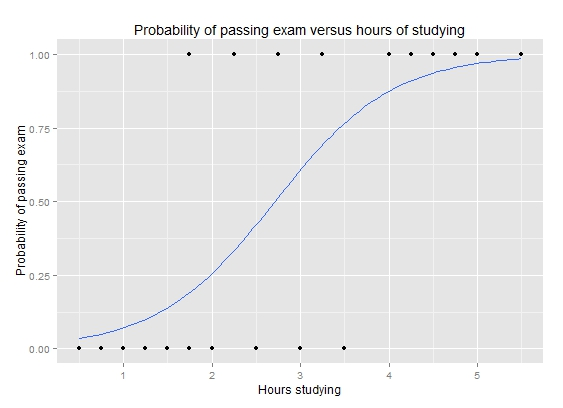
\includegraphics[width=0.8\textwidth]{figures/regression/Exam_pass_logistic_curve.jpeg}
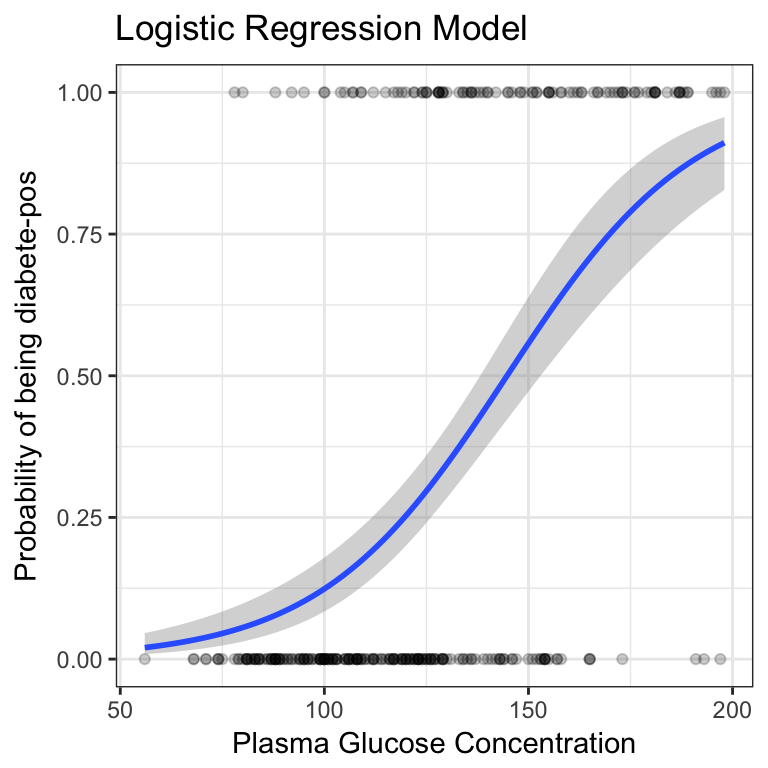
\includegraphics[width=0.8\textwidth]{figures/regression/logistic-regression-probabilities-curve.png}
\caption{
% Example logistic regression curve on one input feature, by \href{https://en.wikipedia.org/wiki/File:Exam_pass_logistic_curve.jpeg}{Michaelg2015}.
Example logistic regression curve on one input feature, by \href{http://www.sthda.com/english/articles/36-classification-methods-essentials/151-logistic-regression-essentials-in-r/}{Kassambara}.
}
\label{fig:logistic_regression_ex}
\end{figure}

Some assumptions of the logistic regression approach are:
\begin{enumerate}[noitemsep]
\item $y$ is either present or absent (dichotomous).
\item There are minimal correlations between the $x_{j}$ features (no multicollinearity).
\item There are no major outliers in the data.
\end{enumerate}

% TODO pseudo R2, Wald statistic

%%%%%%%%%%%%%%%%%%%%%%%%%%%%%%%%%%%%%%%%%%%%%%%%%%%%%%%%
%%%%%%%%%%%%%%%%%%%%%%%%%%%%%%%%%%%%%%%%%%%%%%%%%%%%%%%%
\section{Gaussian Process Regression}
\label{Regression:kriging}
% TODO also known as kriging

